\documentclass[11pt,a4paper]{article}
\usepackage{amsmath}
\usepackage{amsfonts}
\usepackage{amssymb}
\usepackage{fullpage}
\usepackage{graphicx}
\usepackage{hyperref}
\usepackage{float}
\usepackage{siunitx}
\usepackage{mathrsfs}
\usepackage{subcaption}
\usepackage{ulem}
\usepackage[dvipsnames]{xcolor}
\usepackage{xcolor,cancel}
\usepackage{tikz}
\usetikzlibrary{shapes.geometric, arrows}
\tikzstyle{startstop} = [rectangle, rounded corners, minimum width=3cm, minimum height=1cm,text centered, draw=black, fill=red!30]
\tikzstyle{io} = [trapezium, trapezium left angle=70, trapezium right angle=110, minimum width=3cm, minimum height=1cm, text centered, draw=black, fill=blue!30]
\tikzstyle{process} = [rectangle, minimum width=3cm, minimum height=1cm, text centered, draw=black, fill=orange!30]
\tikzstyle{decision} = [diamond, minimum width=3cm, minimum height=1cm, text centered, draw=black, fill=green!30]
\tikzstyle{arrow} = [thick,->,>=stealth]
\newcommand\hcancel[2][black]{\setbox0=\hbox{$#2$}%
\rlap{\raisebox{.45\ht0}{\textcolor{#1}{\rule{\wd0}{1pt}}}}#2}
\usepackage[framemethod=tikz]{mdframed}
\usepackage{lipsum}

\definecolor{mycolor}{rgb}{0.122, 0.435, 0.698}

\newmdenv[innerlinewidth=0.5pt, roundcorner=4pt,linecolor=mycolor,innerleftmargin=6pt,
innerrightmargin=6pt,innertopmargin=6pt,innerbottommargin=6pt]{mybox}

\begin{document}
	\title{NUMERICAL AND COMPUTATIONAL METHOD IN RESEARCH - PYL800\\
	Indian Institute of Technology - Delhi \\
	Assignment - 1}
	
	\author{Course Instructor: Dr. Sujin B Babu \\ 
	Submitted by: Apoorav Singh Deo - \textbf{2021PHZ8046} }
	\maketitle
	

\section*{Strategy}	

To work out the given problem, as in this case Root of the equation (\ref{eq:1}) is to be found. First parameters for the equation are needed to be worked out.

	\begin{figure}[H]	
	\begin{center}
	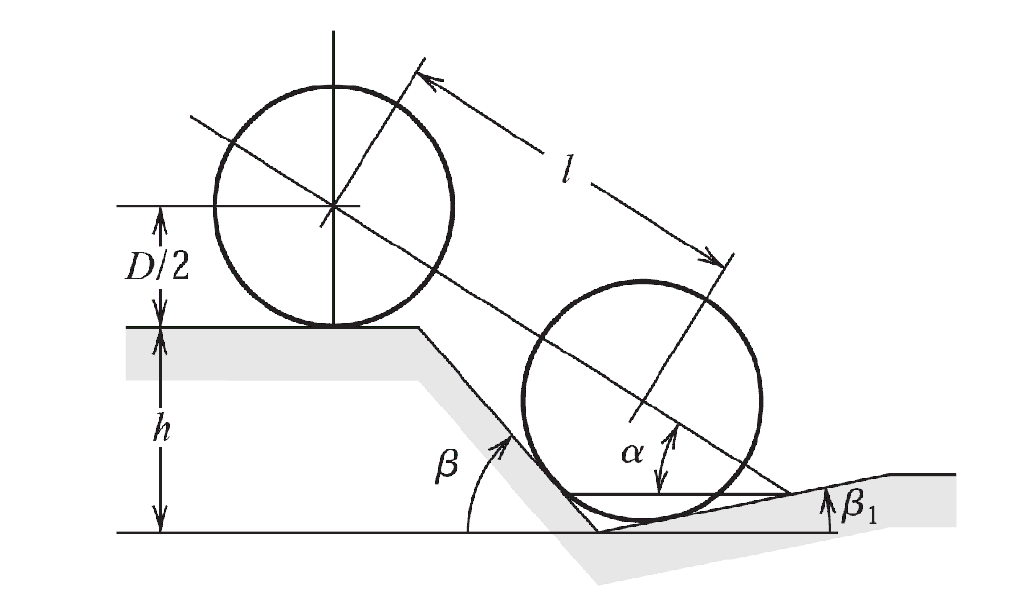
\includegraphics[width=0.5\textwidth]{problem_fig.png}
	\caption{}
	\label{fig:1}	
	\end{center}
	\end{figure}

Parameters such as $l$ = 80 in, $h$ = 40 in, $\beta_1$ = $11.5^o$, $\beta$  is the
maximum angle at which hang-up failure does not occur satisfies the equation (\ref{eq:1}) and $D$ = 30 - 100 in are constant for the computation. $\alpha$ can be varied to see the behavior of the equation. As it can be deduced from the figure (\ref{fig:1}) that at most value that can by the variable $\mathbf{\alpha}$ is not more that $90^o$ and not less than $0^o$. Therefore, this can be our starting point for the iteration.\medskip

Plan would be simple in this computation. First, user would be giving the value to the Bisection algorithm in the code, starting with b = $90^o$ and a = $0^o$. The equation that would be solved using bisection is given as equation (\ref{eq:1})

\begin{align} \label{eq:1}
f(\alpha) = A\sin(\alpha)\cos(\alpha) + B\sin^2(\alpha) - C\cos(\alpha) - E\sin(\alpha)
\end{align}

Program would give certain value of $c$. It will be our wish to work out till what point user want \textit{bisection method} to run before it stops to give its value to next algorithm i.e. \textit{newton-raphson method}, which just requires one value to initiate the computation and would converge to the nearest root. To work out the second method derivative function is needed, which is manually derived (equation (\ref{eq:2})).

\begin{align} \label{eq:2}
f'(\alpha) = A\cos(2\alpha) + B\sin(2\alpha) + C\sin(\alpha) - E\cos(\alpha)
\end{align}

The results could be stored in the variable after each computation i.e. for every value of \textbf{D}. As asked, curve can be plotted between $\alpha$  where $f(\alpha) = 0$ versus corresponding value of \textbf{D}.

\subsection*{Bisection Method}

First and foremost task was to check if function is analytic or not. So I plotted the function to get an rough idea of it as well as to see if there is not any singularities. As it can be seen in the figure (\ref{fig:2}), function is analytic and root of the function lies between $20^o$ and $40^o$. For other values of \textbf{D} nature of graph is not changed.

	\begin{figure}[H]	
	\begin{center}
	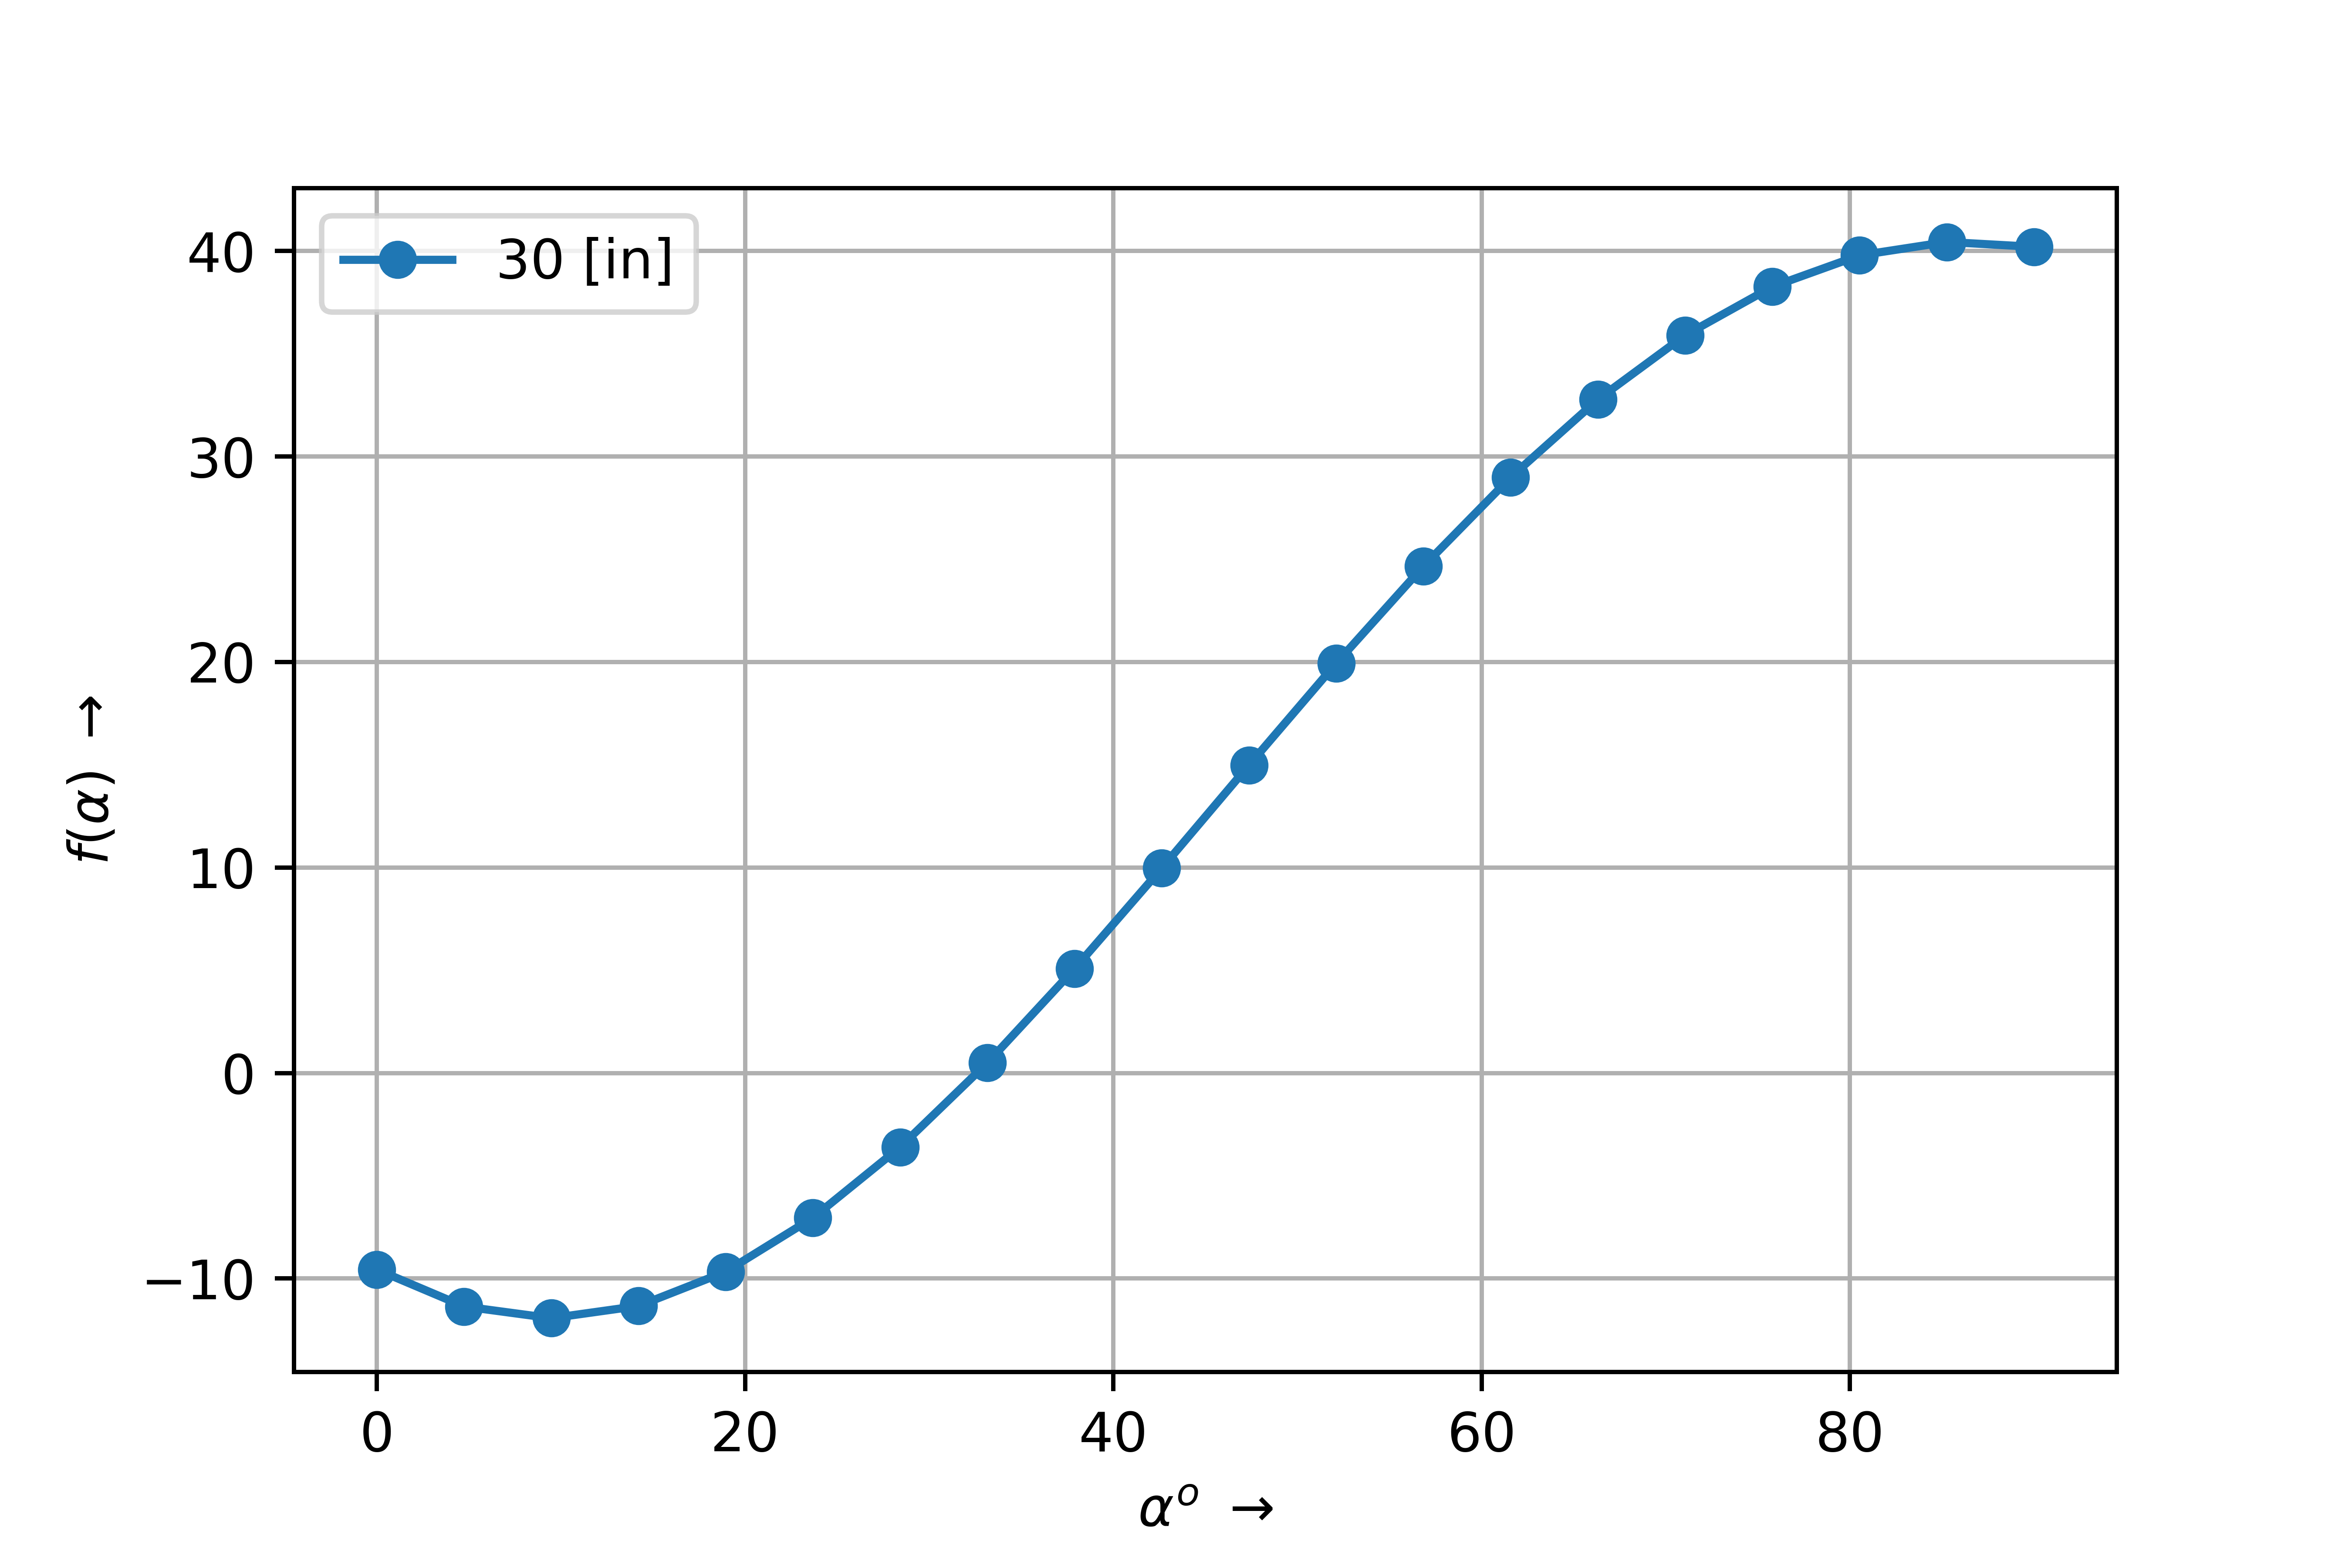
\includegraphics[width=0.5\textwidth]{func_1.png}
	\caption{Plot for equation (\ref{eq:1})}
	\label{fig:2}	
	\end{center}
	\end{figure}

Now, implementation of the \textit{bisection method} is pretty simple.

\begin{enumerate}
\item $f(a)\times f(c) < 0$: Root lies between \textbf{a} and \textbf{c}. Therefore, \textbf{b} would be swapped with \textbf{c}
\item $f(b)\times f(c) < 0$: Root lies between \textbf{a} and \textbf{c}. Therefore, \textbf{a} would be swapped with \textbf{c}
\end{enumerate} 
 
I am limiting the bisection code to just 2 iteration. Although it is completely dependent on the user what value to choose (I have not included user input for the same as for now it was not necessary). Now, a value of \textbf{c} which is generated by the calculation would be fed to next algorithm.

\subsection*{Newton Raphson Method} 

To work out this algorithm, first thing is to be checked if the derivative of equation (\ref{eq:1}) is not zero in the given domain i.e. where we are going to run the calculation.\medskip

Therefore, plot of equation (\ref{eq:2}) is made in figure (\ref{fig:3}). According to the plot our calculation should not exceed $60^o$ or so. Although root lies below $40^o$ mark. Hence, it is safe to move ahead.

	\begin{figure}[H]	
	\begin{center}
	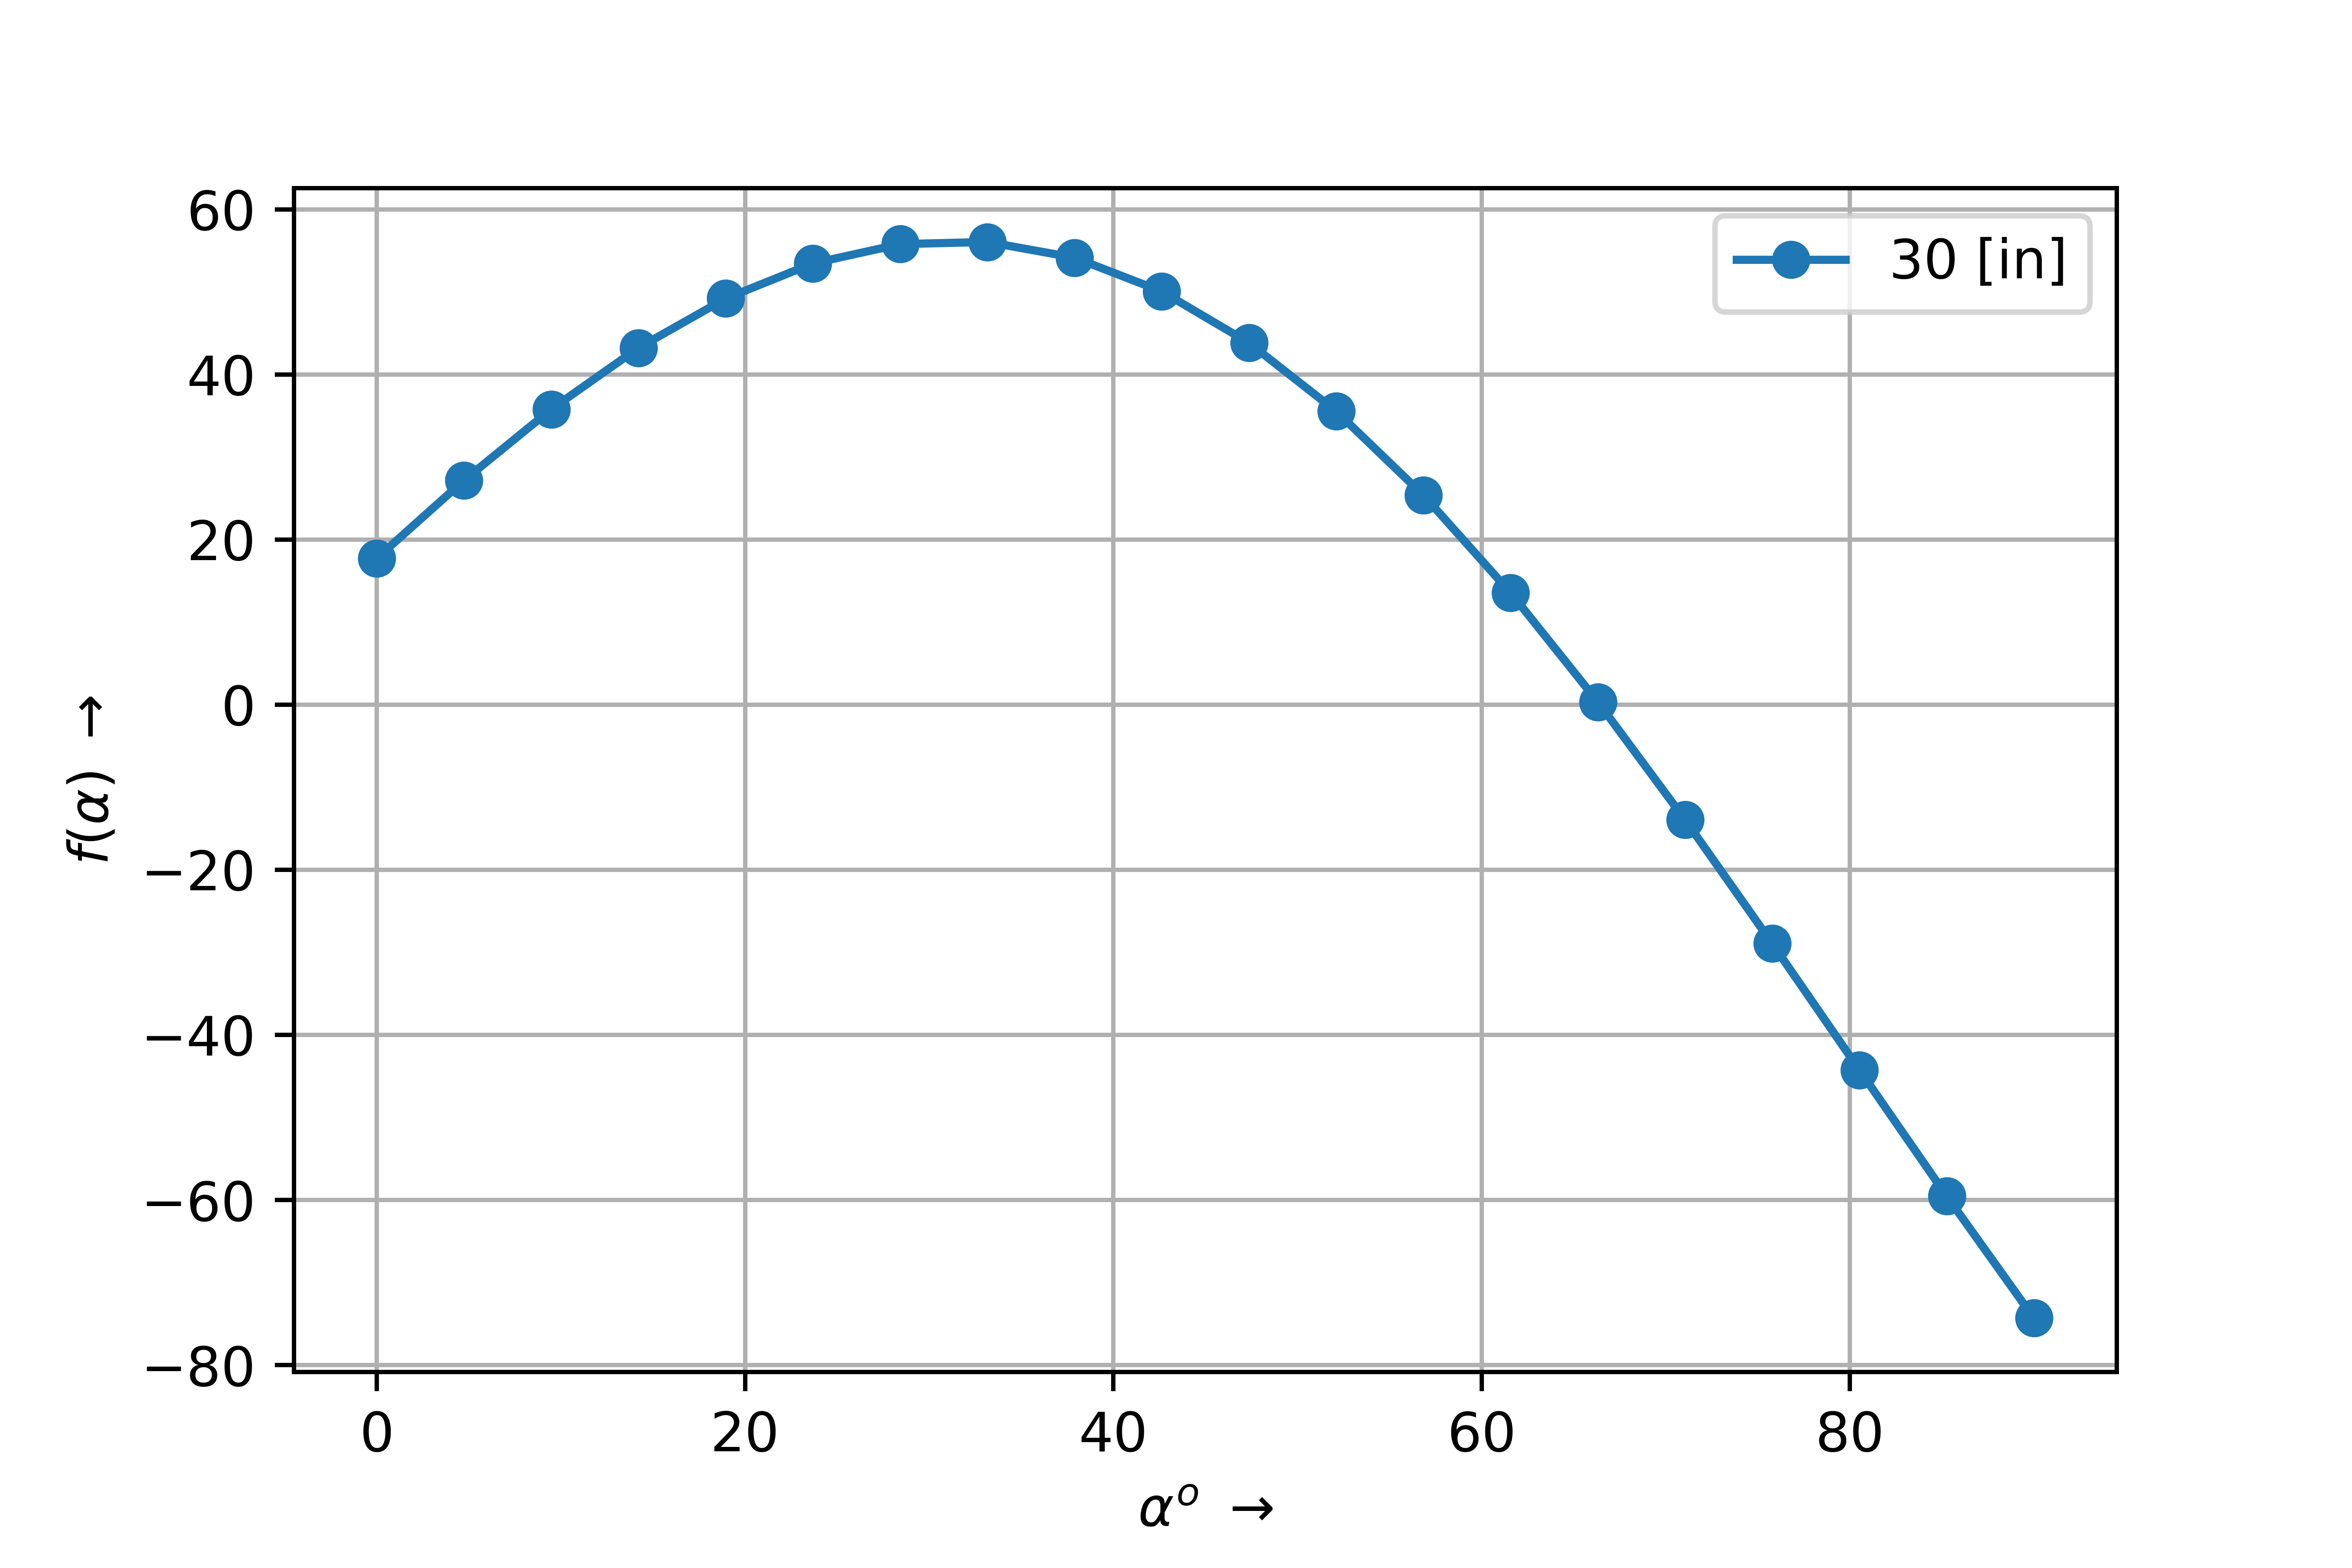
\includegraphics[width=0.5\textwidth]{func_2.png}
	\caption{Plot for equation (\ref{eq:2})}
	\label{fig:3}	
	\end{center}
	\end{figure}

Implementation of the algorithm  is pretty simple, it is as one would do manual calculation. Just implement the formula.

\begin{align*}
x_{i+1} = x_{i} - \left[\frac{f(x_i)}{f'(x_i)}\right]
\end{align*}

Just after that  step $x_{i}$ can be swapped with $x_{i+1}$. This algorithm is made to run inside a while loop. The condition for termination of the while loop is the point when $f(\alpha)\ < \ tolerance $.

\subsection*{Values of D}

This whole process runs under the shade of single \textbf{D} value. Which in turn iterates from its beginning value to end value. Along with these values $\alpha$ where function is deemed zero is mapped in an array and plotted as seen in the figure (\ref{fig:4}) 

	\begin{figure}[H]	
	\begin{center}
	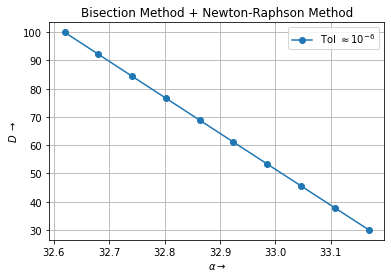
\includegraphics[width=0.5\textwidth]{Bisection_Method.png}
	\caption{\textbf{D} versus $\alpha$ }
	\label{fig:4}	
	\end{center}
	\end{figure}

From the graph it can be concluded that diameter of the Tyre has linear relationship with $\alpha$ for which hang-up failure does not occur.

\section*{Code Implementation}

The code is written in python 3.9 . The code goes as follows:

\begin{mybox}
\begin{verbatim} 
# Assignment 1 - (PYL800)
# Code By: Apoorav Singh Deo 
# En. Number: 2021PHZ8046

import math 
import numpy as np

from matplotlib import pyplot as plt

# [Parameters]
l = 89.0 # [inches]
beta_1 = 11.5*(math.pi/180) # [radians]
h = 49.0 # [inches]


# Function Implementation

def func_1(alpha, D):
    A = l*math.sin(beta_1)
    B = l*math.cos(beta_1)
    C = (h + 0.5*D)*math.sin(beta_1) - 0.5*D*math.tan(beta_1)
    E = (h + 0.5*D)*math.cos(beta_1) - 0.5*D
    y = A*math.sin(alpha)*math.cos(alpha) + \\
     B*(math.sin(alpha))**2 - C*math.cos(alpha) - E*math.sin(alpha)

    return y

# Function Derivative Implementation

def func_2(alpha, D):
    A = l*math.sin(beta_1)
    B = l*math.cos(beta_1)
    C = (h + 0.5*D)*math.sin(beta_1) - 0.5*D*math.tan(beta_1)
    E = (h + 0.5*D)*math.cos(beta_1) - 0.5*D
    y = A*math.cos(2*alpha) + B*(math.sin(2*alpha)) - \\
     C*math.sin(alpha) - E*math.sin(alpha)

    return y

# Algorithm for Bisection method

# Initial guess is taken to be as 0 and 1
print("\t Bisection Method")
print("\n")
print(r"$\theta_i = 0^o and \theta_f = 90^o$")
print("\n")

n1 = 10 # Number of Iterations for D
i = 0 # Iteration Variable 


dump_c = np.empty(n1)
# Would store the value of the last value of c i.e. c = (a+b)/2
# For each iteration 

dump_f_c = np.empty(n1)
# Would store the value of the last value of f(c)
# For each iteration

alpha = np.empty(n1)


tol = 1e-6 # Tolerace limit

D_range = np.linspace(30, 100, n1) # units [in]

for D in D_range:
    
    j = 0 # Help in breaking the loop at desired point.
    
    print("Running for D = {}".format(D))
    print("\n")
    
    a = 0*(math.pi/180)
    b = 90*(math.pi/180)

    
    
    #f_a = func_1(a, D)
    #f_b = func_1(b, D)
    
    c = (b+a)*0.5
    f_c = func_1(c, D)
    

# Redeclaration of the 'c' and 'f_c' is 
#done to compute the values inside the loop
    
    while (abs(f_c) >= tol):
        
        c = abs((b+a)*0.5)
        f_c = func_1(c, D)
        
        f_a = func_1(a, D)
        f_b = func_1(b, D)
        
        if ((f_a*f_c)<0 and (f_b*f_c)>0):
            b = c
        
            
        elif ((f_a*f_c)>0 and (f_b*f_c)<0):
            a = c
        
        if (j == 10):
            break
        
        j += 1 
        #print(c*(180/math.pi),f_c)
    
# Algorithm for Newton-Raphson Method
    
    while (abs(f_c) >= tol):
        
        x = c - (func_1(c, D)/func_2(c, D))
        c = x
        f_c = func_1(c, D)
        print(c*(180/math.pi),f_c)
        
                
            
    #print(k)
    dump_f_c[i] = f_c
    dump_c[i] = c    
    
    alpha[i] = (180/math.pi)*dump_c[i]
    
    i += 1
    print("\n")
        
plt.plot(alpha, D_range, marker='o', label=r'Tol $\approx 10^{-6}$')
plt.legend()
plt.xlabel(r"$\alpha \rightarrow$")
plt.ylabel(r"$D\ \rightarrow$")
plt.grid(True)
plt.title("Bisection Method + Newton-Raphson Method")
plt.grid(which='minor')
plt.show()

plt.savefig("Bisection_Method.png", dpi=900)
\end{verbatim}
\end{mybox}

\subsection*{Running the code}

[\texttt{For Windows}] Anaconda distribution\footnote{\url{https://www.anaconda.com/products/individual}} don't need any dependency to be installed. One can simply run the code in it using any one of the IDEs in it. (Spyder is suggested).\medskip

[\texttt{For Linux}] Terminal can also be used to execute this code, but make sure dependencies are installed before hand. These dependencies can be installed using  \texttt{pip}.\footnote{\url{https://pip.pypa.io/en/stable/}}. Type in these commands in the BASH terminal after installing pip.

\begin{enumerate}
\item \texttt{pip install matplotlib}
\item \texttt{pip install numpy}
\item \texttt{pip install scipy}
\end{enumerate}

To execute the program run command on the BASH terminal:
\begin{verbatim}
>> python3 file_name.py
\end{verbatim}

\section*{Reference}

\begin{enumerate}
\item Class Notes.
\item \url{https://numpy.org/doc/stable/}
\item Tutorial by Corey Schafer [Matplotlib]
\item \url{https://matplotlib.org/stable/gallery/index.html}
\item \textbf{Numerical Analysis} by \texttt{Richard L. Burden and J. Douglas Faires} 
\end{enumerate}




\end{document}
